\documentclass{article}
\usepackage{graphicx} 
\usepackage{caption}
\usepackage{geometry}
 \geometry{
 a4paper,
 total={170mm,257mm},
 left=20mm,
 top=20mm,
 }
 
\title{Bouton d'arrêt d'urgence}
\author{Cyril Hérail}
\date{An de grâce 2023}

\begin{document}

\maketitle

 Le bouton d'arrêt d'urgence est un élément de sécurité important du robot et nécessaire à son homologation. 

\section*{Rappel des consignes}

Le règlement de la CDR 2024 impose la présence d'un bouton d'arrêt d'urgence. Ce dernier précise que le bouton d'arrêt d'urgence doit:

\begin{itemize}
    \item faire \textbf{au minimum} 20mm de diamètre
    \item être "au sommet du robot"
    \item facilement accessible
    \item être "visible"
    \item être sur une surface "libre"
\end{itemize} 

\section*{Rappel sur les boutons}

Un bouton est dit \textbf{normalement ouvert} (NO), s'il ne conduit pas lorsque n'on appuie pas dessus. Il conduit lorsque l'on appuie sur le bouton. \\
Un bouton est dit \textbf{normalement fermé} (NF), s'il conduit lorsque l'on n'appuie pas dessus. Il ne conduit pas lorsque l'on appuie sur le bouton.

\section*{Matériel présent}

On a au local deux boutons d'arrêt d'urgence identique, utilisés lors des CDR des années précédentes. Ils ont un diamètre de 40mm, ce qui est plus que nécessaire. Au niveau de l'ampérage, il est important de préciser qu'ils supportent \textbf{au maximum 10A}. \\

\begin{figure}[h]
    \begin{minipage}{0.45\textwidth}
        \centering
        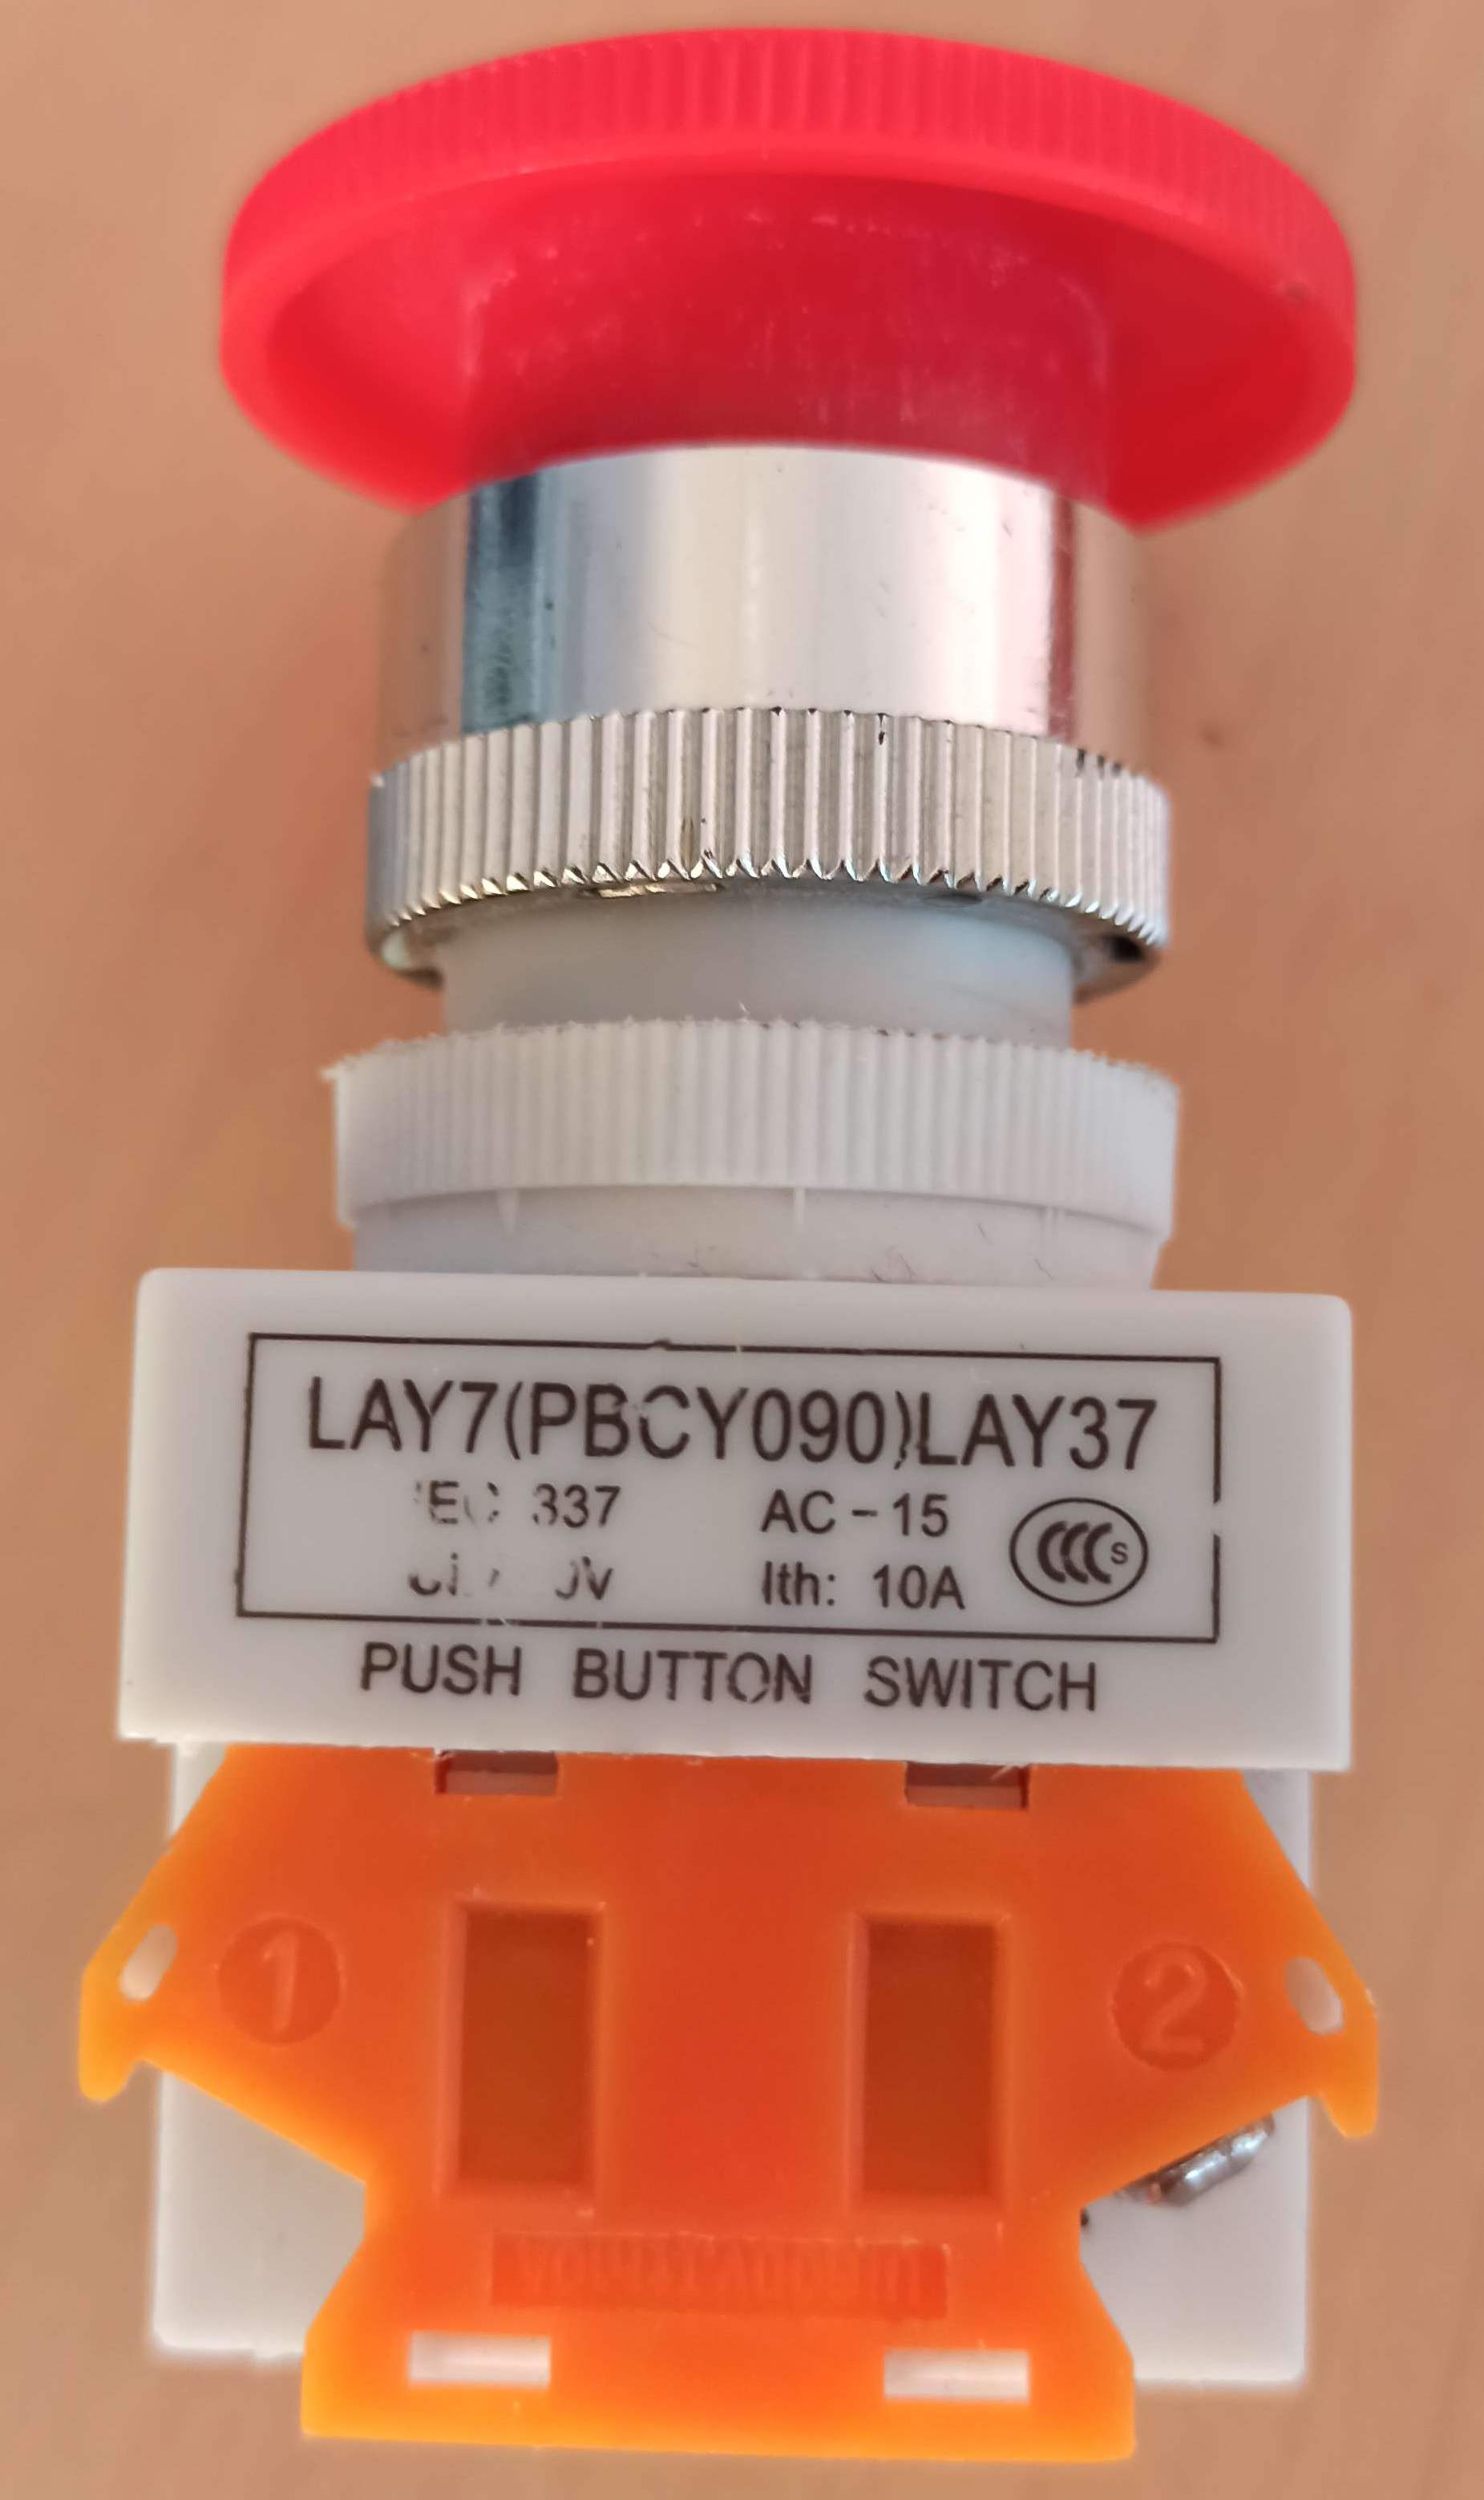
\includegraphics[width=0.5\linewidth]{images/bouton_vue_generale_1.jpg}
        \captionsetup{labelformat=empty}
        \caption{}
        \label{fig:image1}
    \end{minipage}
    \hfill
    \begin{minipage}{0.45\textwidth}
        \centering
        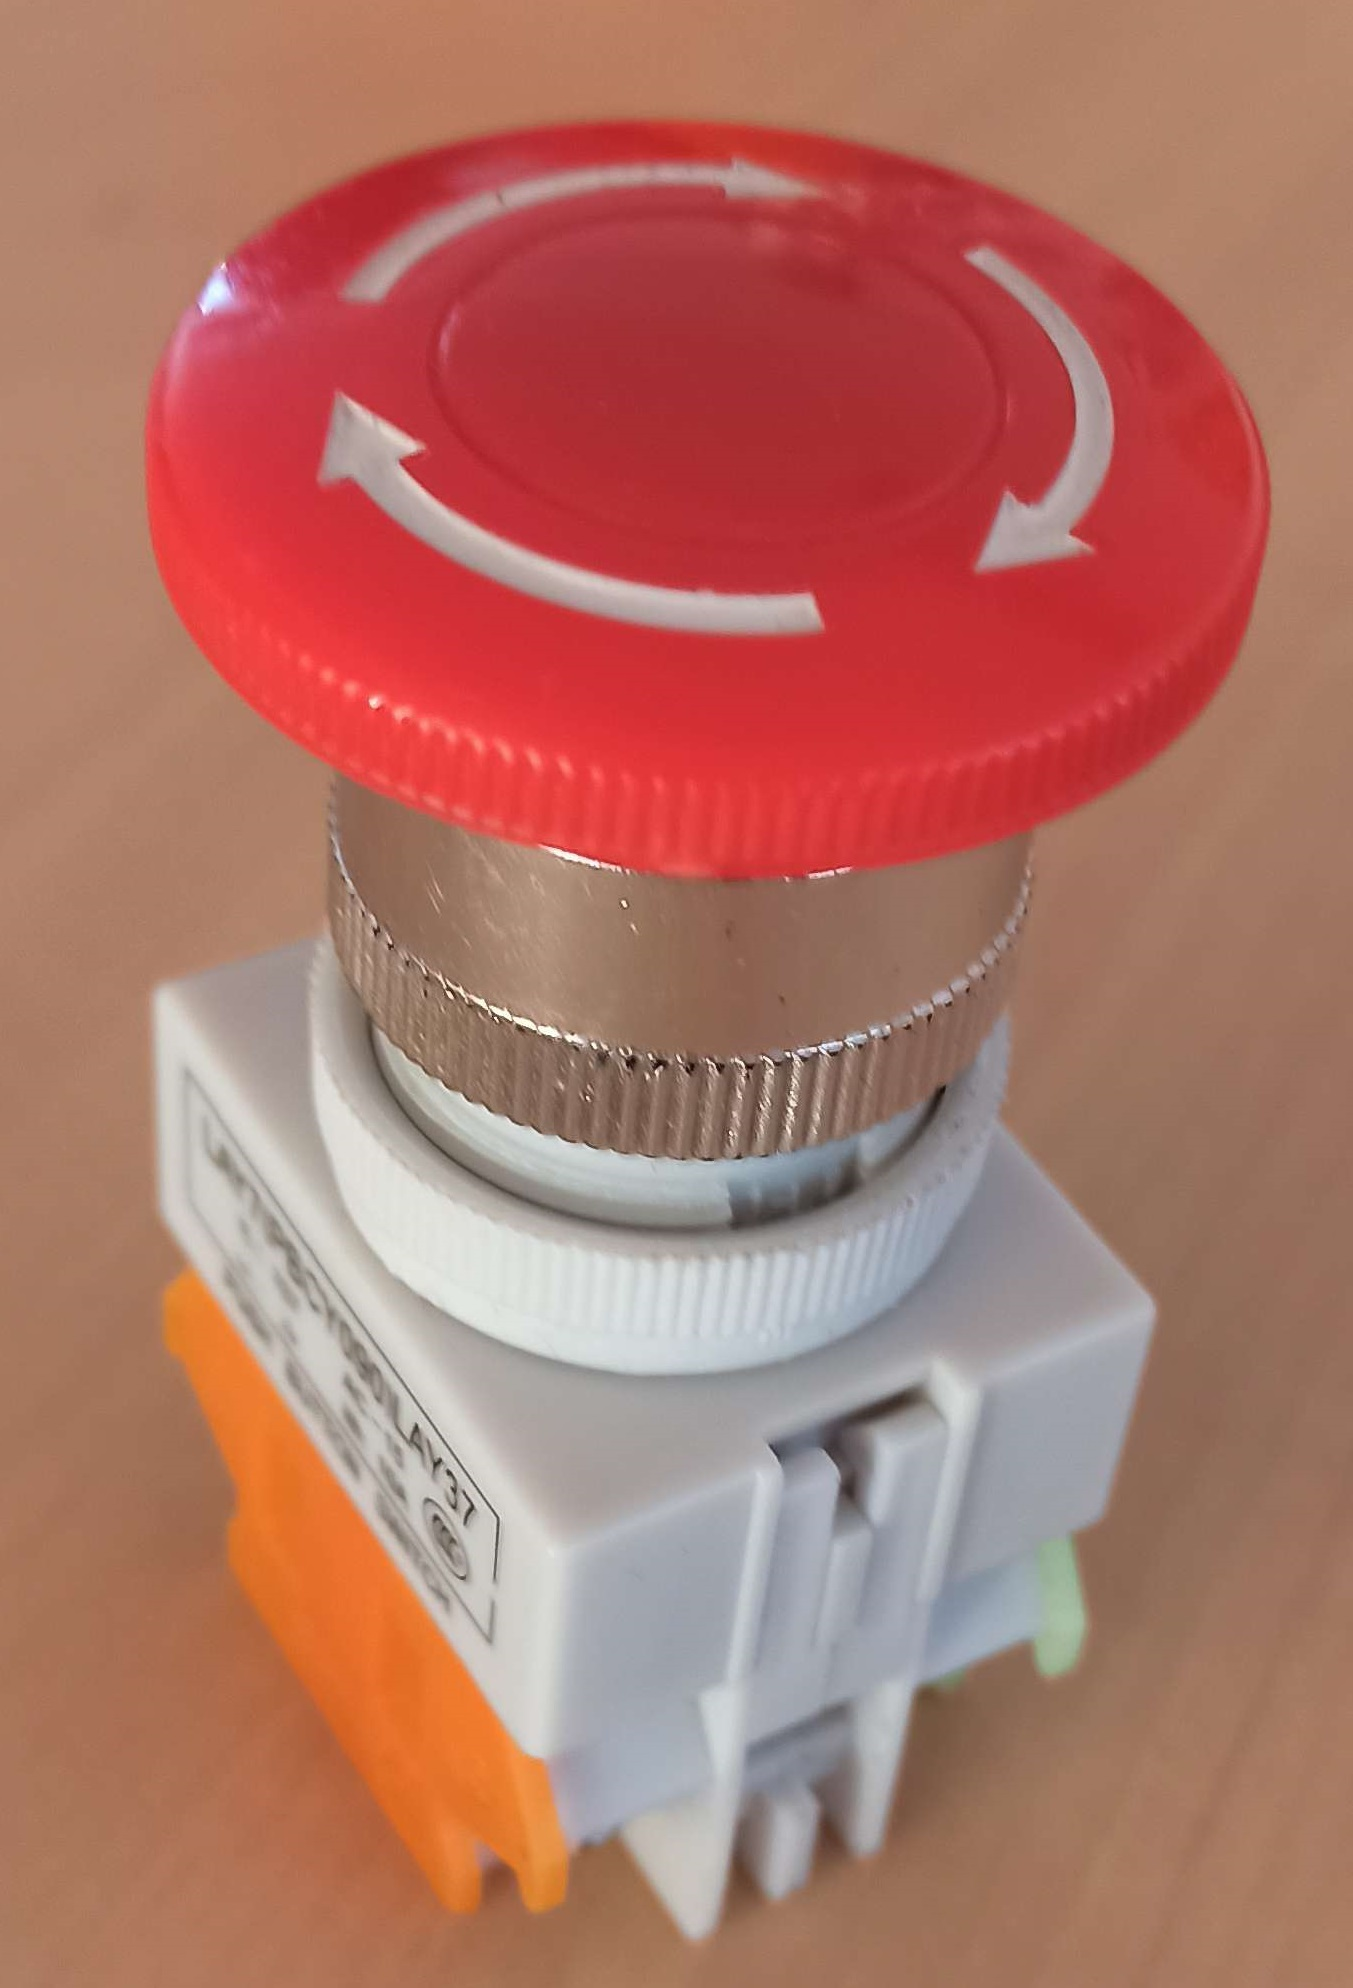
\includegraphics[width=0.5\linewidth]{images/bouton_vue_generale_2.jpg}
        \captionsetup{labelformat=empty}
        \caption{}
        \label{fig:image2}
    \end{minipage}
\end{figure}

Comme vous pouvez le voir sur les photos, ils ont un côté vert et un côté orange. 

\newpage
A l'intérieur du bouton, les deux côtés ne sont pas reliés. Aussi, le côté vert est de type NO, le côté orange est de type NF. Lorsque vous allez appuyer sur le bouton, le courant traversant le côté orange va être bloqué tandis que le courant côté vert va pouvoir circuler.

\begin{figure}[h]
    \begin{minipage}{0.6\textwidth}
        \centering
        \rotatebox{-90}{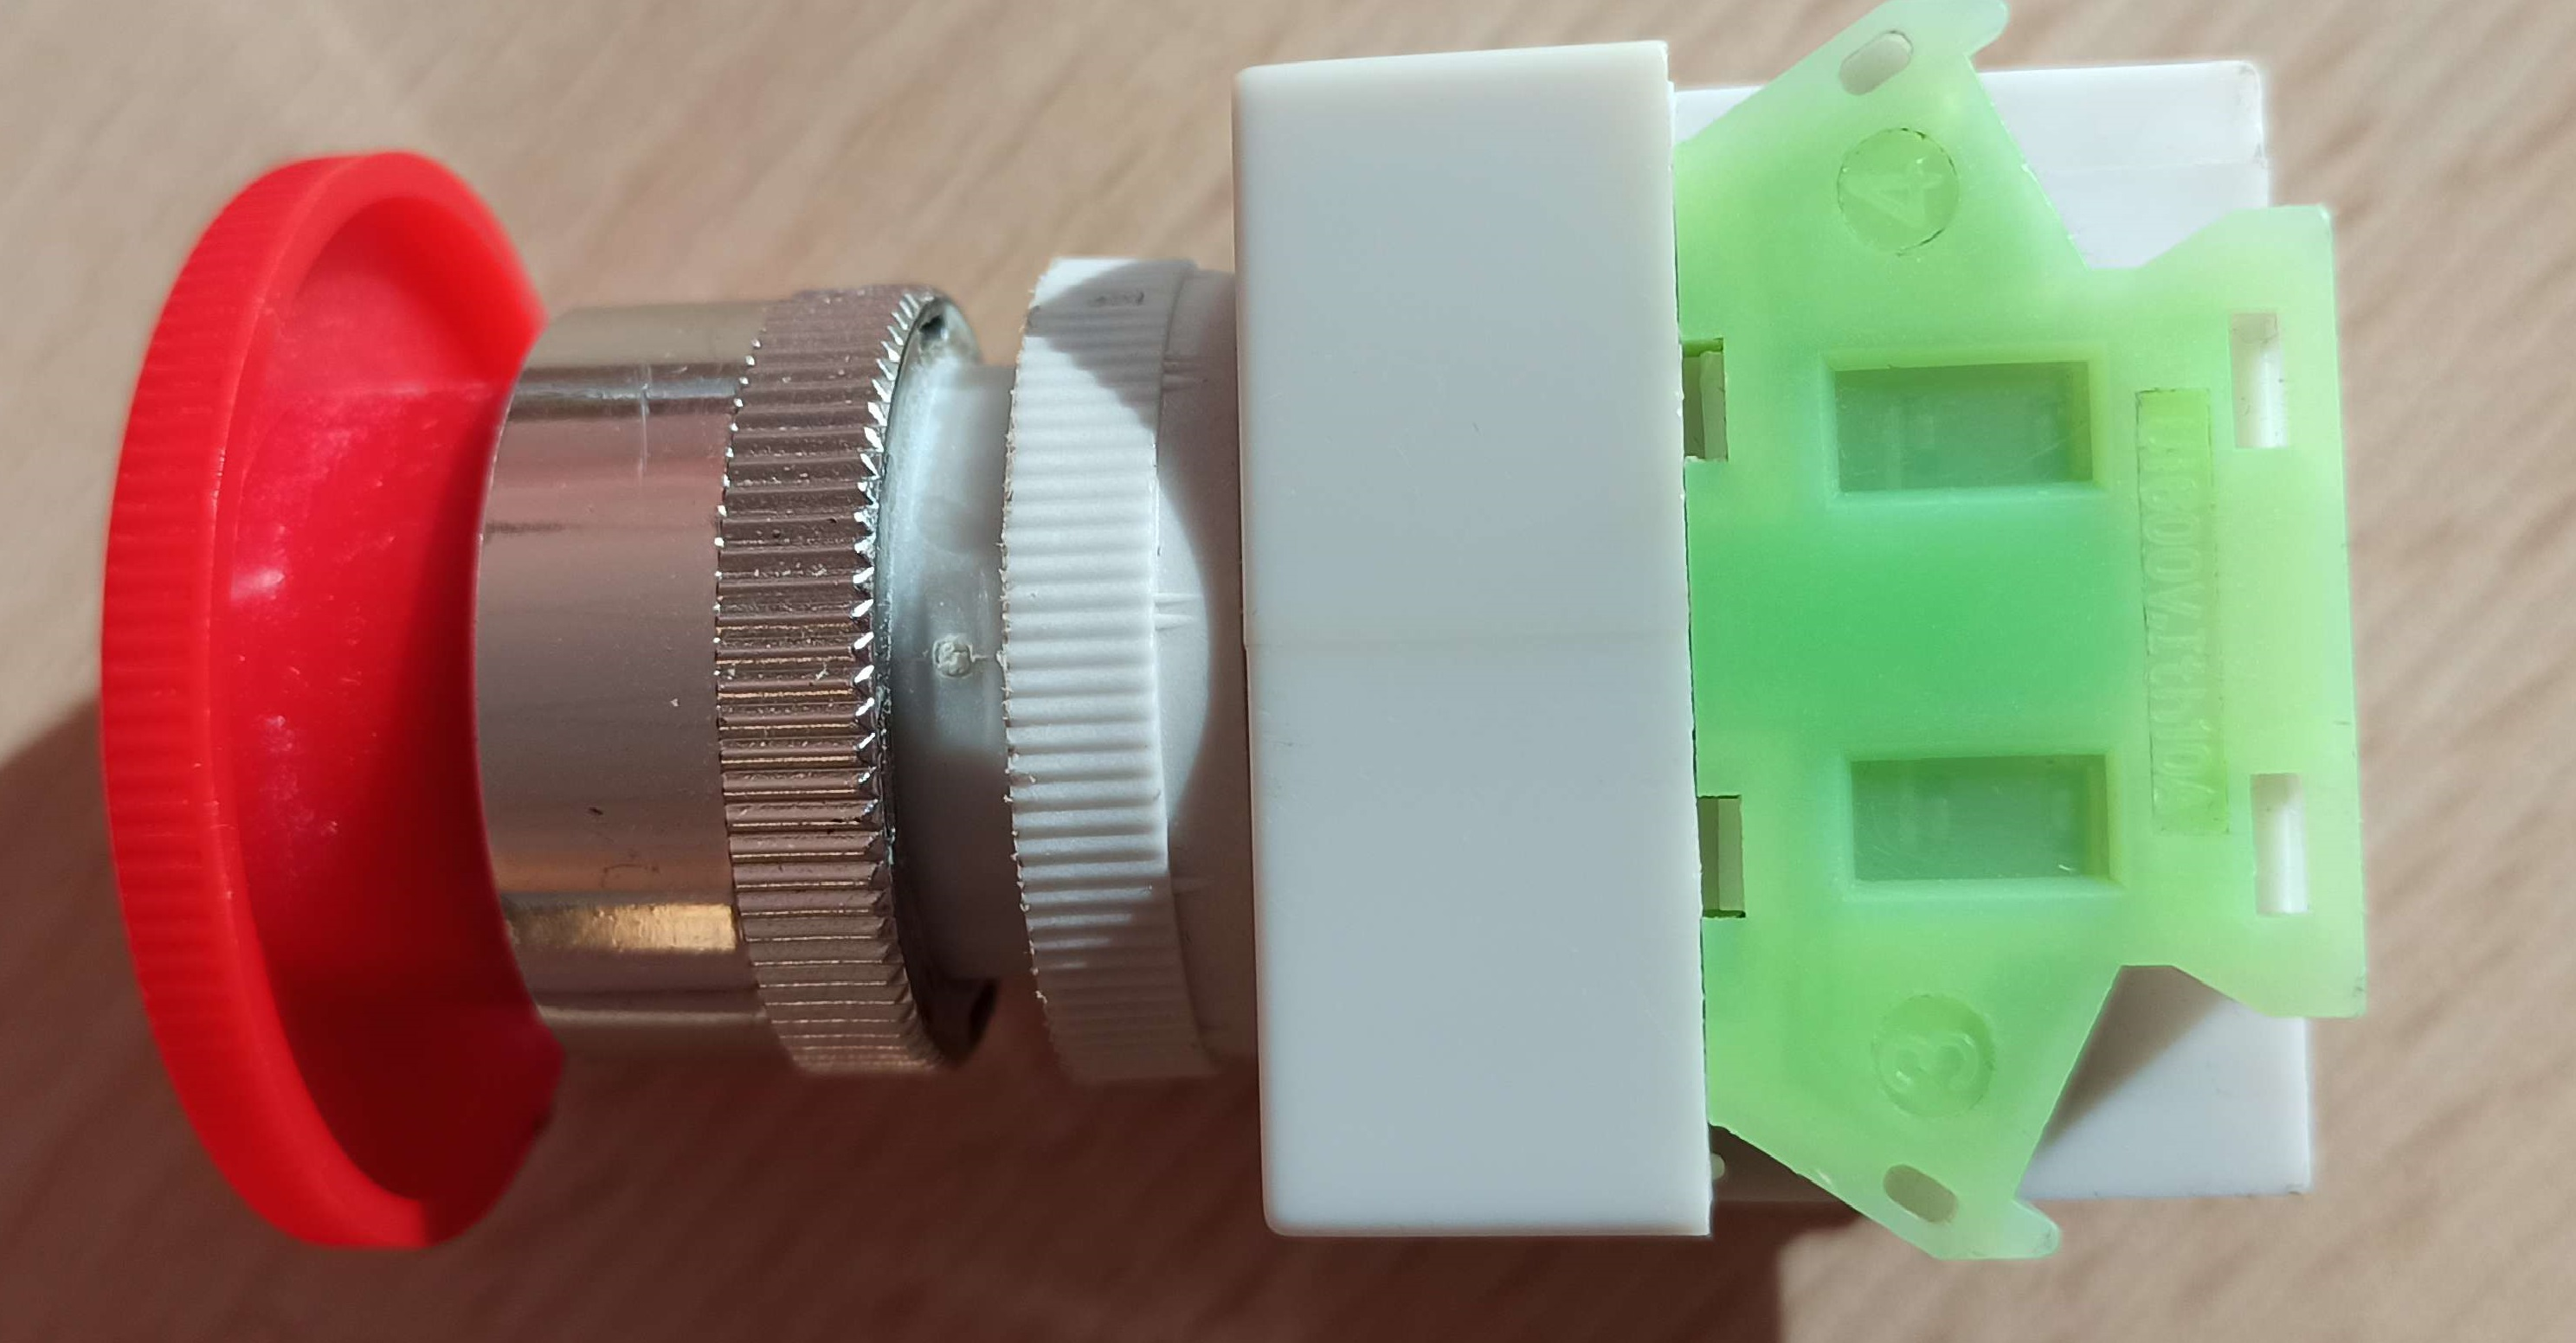
\includegraphics[width=\linewidth]{images/bouton_vert_ouvert.jpg}}
        \captionsetup{labelformat=empty}
        \caption{bouton non enclenché}
    \end{minipage}
    \hfill
    \begin{minipage}{0.45\textwidth}
        \centering
        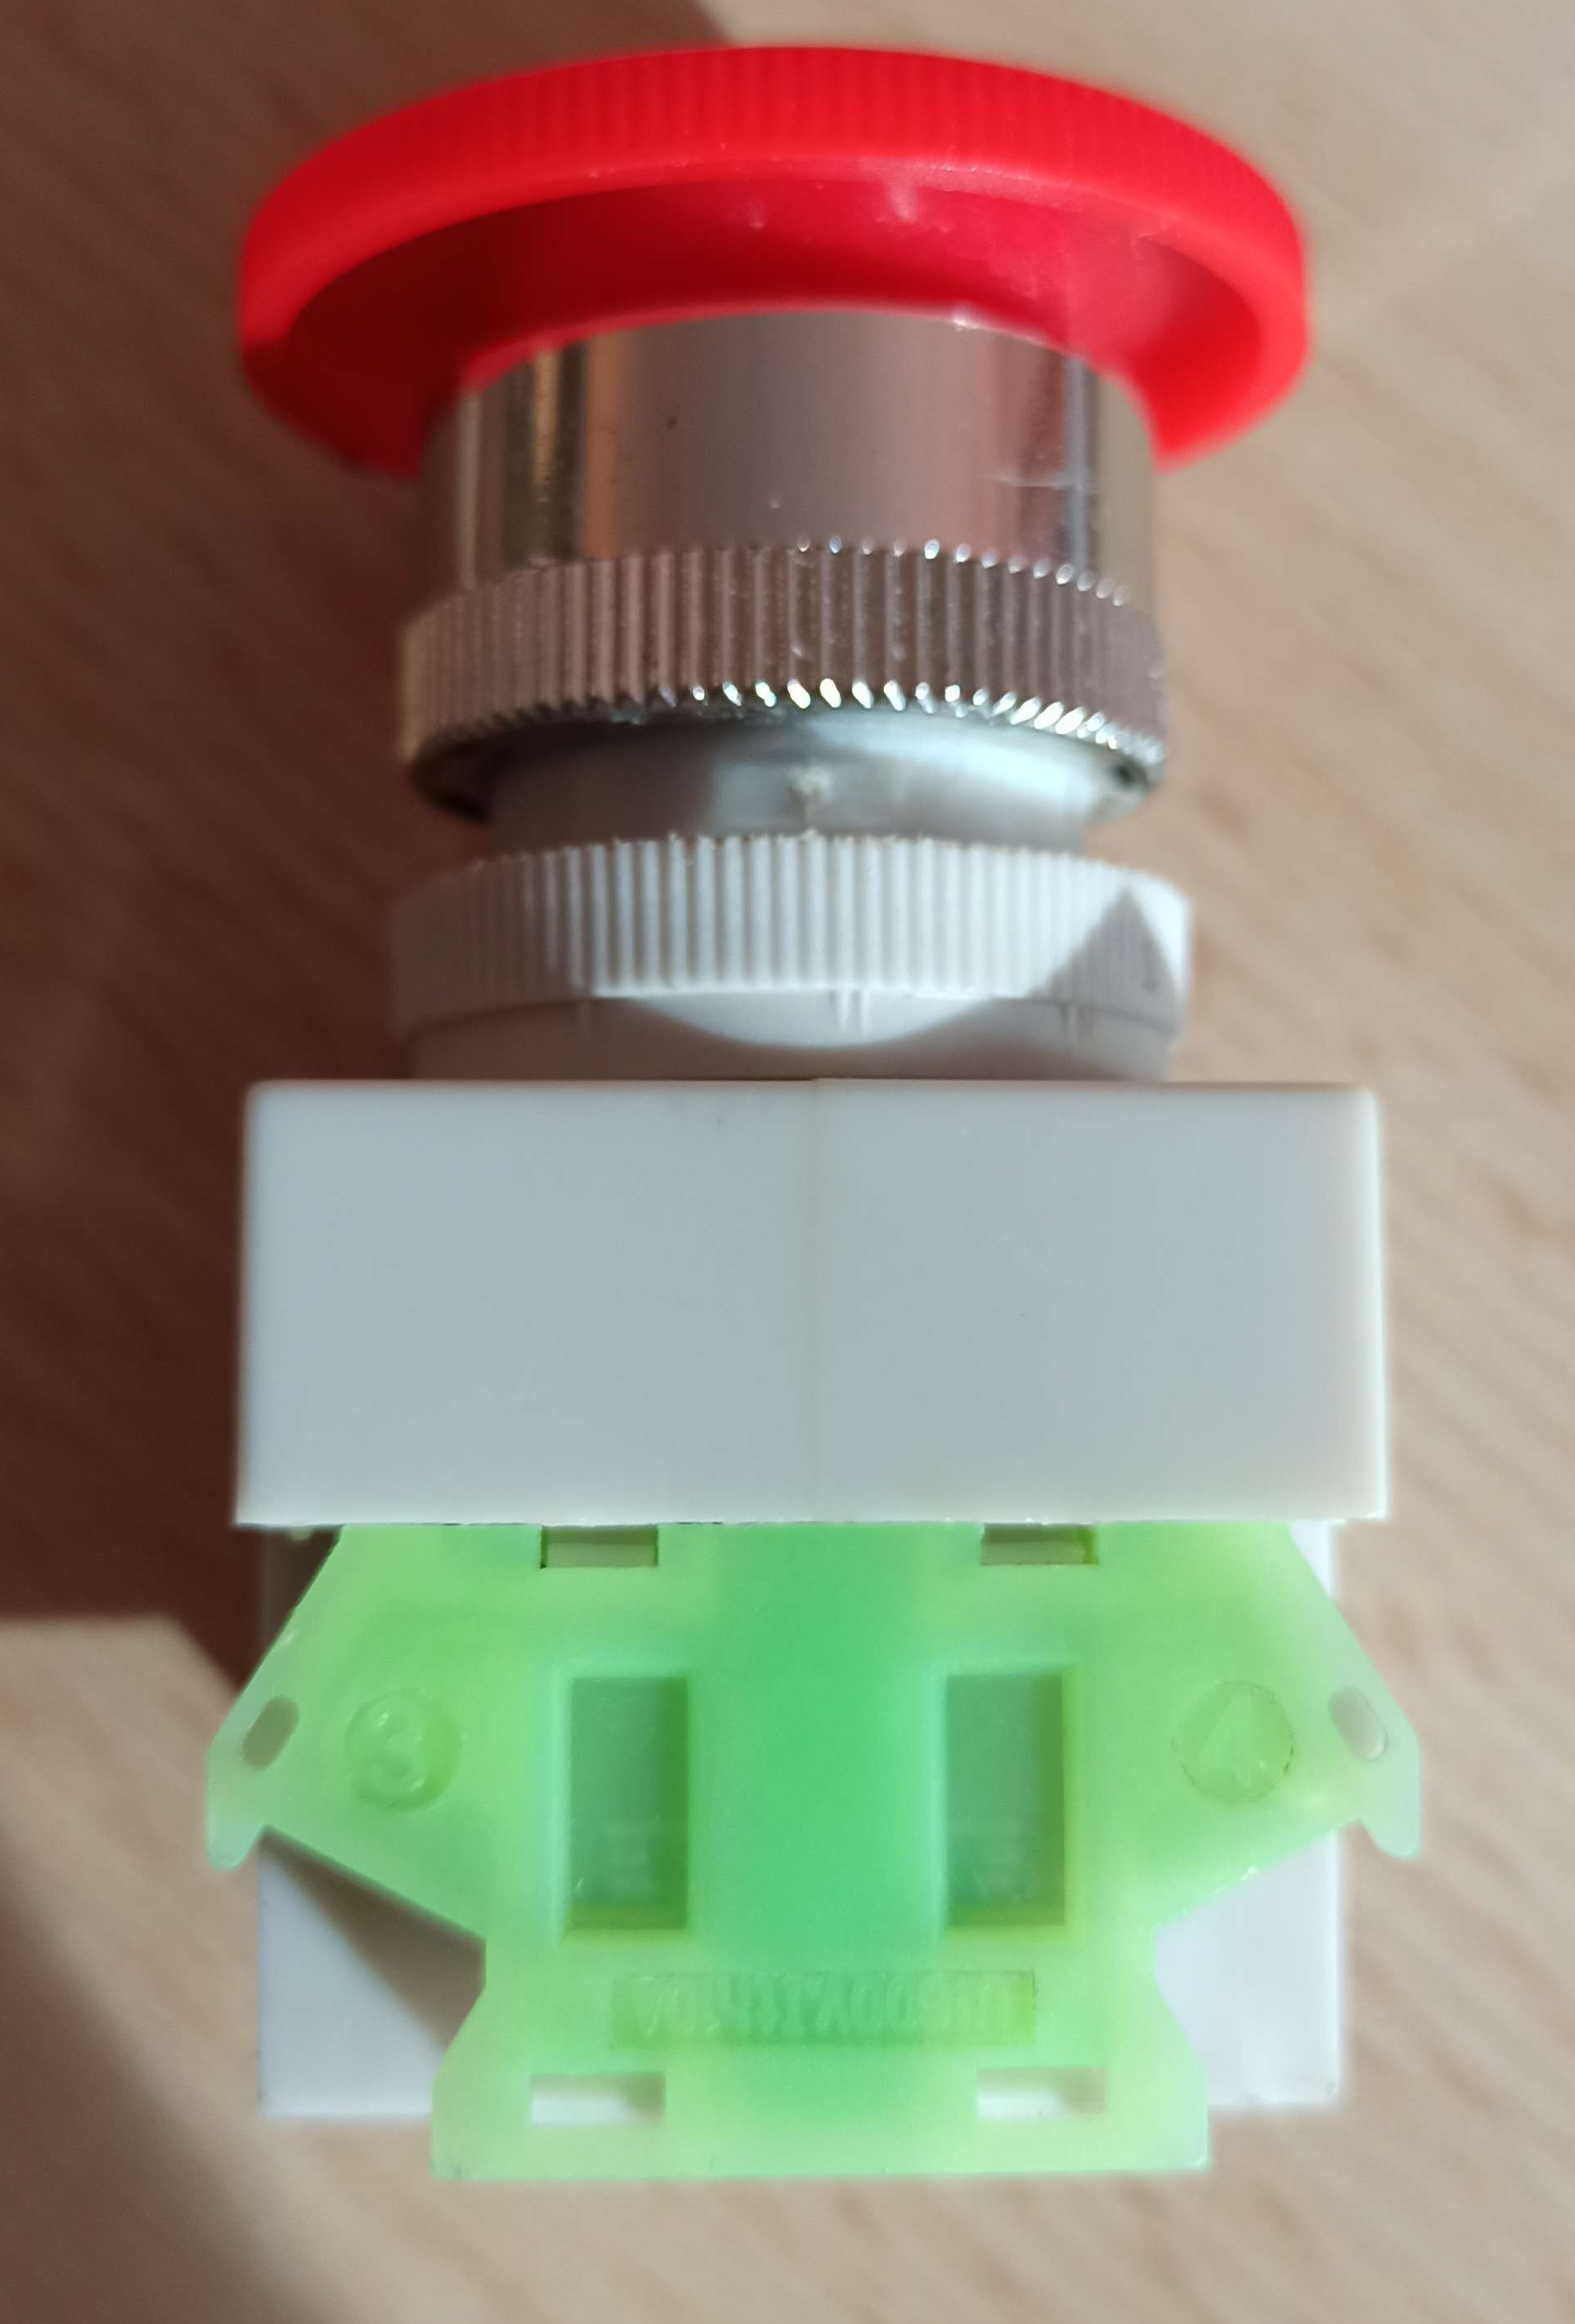
\includegraphics[width=0.9\linewidth]{images/bouton_cote_vert_ferme.jpg}
        \captionsetup{labelformat=empty}
        \caption{bouton enclenché}
    \end{minipage}
\end{figure}

D'ailleurs, plutôt que d'utiliser un multimètre, vous pouvez directement regardez sur les côtes pour voir si c'est un un côté NO ou un côté NF. Regardez bien les photos!


\end{document}
